\documentclass{../../../oss-handout}
\usepackage{amsmath,bm}
\usepackage{txfonts}  % must be loaded after amsmath?
\usepackage{enumitem}
\usepackage{tikz}
\usepackage{siunitx}

\sisetup{
  detect-all,
  per-mode=symbol
}

%\usetikzlibrary{decorations.pathmorphing,patterns}

\newcommand{\mb}[1]{\mathbf{#1}}
\newcommand{\iii}{\bm{\hat{\imath}}}
\newcommand{\jjj}{\bm{\hat{\jmath}}}
\newcommand{\kkk}{\bm{\hat{k}}}
\newcommand{\pic}[2]{\includegraphics[width=#1\textwidth]{#2}}

\setlength{\parindent}{0pt}
\setlength{\parskip}{8pt}
\setlength{\headheight}{26pt}

% Set the page style for the document
\pagestyle{plain}

% Course & handout information
\renewcommand{\institution}{Olympiads School, Toronto, ON, Canada}
\renewcommand{\coursetitle}{Advanced Placement Physics C}
\renewcommand{\term}{Summer 2020}

\title{Examples of Rigid-Body Rotational Motion}
\author{Timothy M.\ Leung, Ph.D.}
\date{\today}

\begin{document}
\thispagestyle{title}
\gentitle

The case of a rolling sphere is a standard example of combining the dynamics of
translational and rotational motions of a rigid body. In this handout, two
typical examples are be presented for a non-slip (i.e.\ pure rolling) case,
while one example is presented for a case with slippage.

\section{Pure Rolling of Rigid Body on Flat Surface}
\label{no-slip-ball}
In the first case, a smooth solid sphere of constant density rolls on a smooth
surface without slipping (rolling without slippage is called
\textbf{pure rolling}). We assume that the sphere and the surface are both
perfectly rigid, in that they cannot be deformed. We also assume that the sphere
and the surface are both perfectly smooth without defects even at the atomic
level. The free-body diagram is shown in Fig.~\ref{roll-flat}. Notice that
\emph{there is no friction between the sphere and the surface}. Since there is
neither a net force nor a net torque acting on the sphere, neither the
translational nor rotational state of the ball changes over time. In
theory---if our assumptions are correct---a the sphere with translational
velocity $\mb{v}$ and angular velocity $\bm{\omega}$ will roll along forever.
\begin{figure}[!ht]
  \centering
  \begin{tikzpicture}[scale=1.3]
    \tikzstyle{balloon}=[ball color=gray!20];
    \shade[balloon](0,0) circle(1);
    \draw[thick](-2,-1)--(2,-1);
    \draw[thick,->](1.5,0)--(2.5,0) node[pos=1,right]{$\mb{v}$};
    \draw[thick,->](0,1.2) arc(90:60:1.2) node[midway,above]{$\bm{\omega}$};
    \draw[->](4,0)--(5,0) node[pos=1,right]{$x$};
    \draw[->](4,0)--(4,1) node[pos=1,above]{$y$};
    \fill(0,0) circle(.05) node[right]{\small CM};
    \draw[->,ultra thick,blue!80!black](0,0)--(0,-1.5)
    node[pos=1,below]{$\mb{w}$};
    \draw[->,ultra thick,red!80!black](-.03,-1)--(-.03,.5)
    node[pos=1,above]{$\mb{N}$};
  \end{tikzpicture}
  \caption{Force diagram on a uniform density solid sphere rolling on a smooth
    flat surface without slipping.}
  \label{roll-flat}
\end{figure}

\textbf{But of course, we are very observant.} Even a casual observer will
notice that in reality, a ball will slow down and eventually come to a stop. A
steel ball bearing rolling on a track rolls over a much longer distance and
much longer time than a soccer ball on a grassy field, but neither will roll
forever. So what causes this? Specifically, what is missing in the free-body
diagram in Fig.~\ref{roll-flat}?

\textbf{Our assumptions aren't quite correct.} There are two major oversights
in our initial assumptions.
\begin{enumerate}
\item\textbf{Nothing is perfectly smooth.} Firstly, our original assumptions
  mean that the contact area is infinitesimal small, and the normal force, by
  basic geometry, points straight toward the CM. However, we should recognize
  that neither the ball bearing nor the rail are perfectly smooth. When a
  non-smooth ball rolls over a non-smooth surface, their surface roughness
  means that the contact point is finite in size, and that the normal force
  does not necessarily point toward the CM of the ball. This means that unlike
  in Fig. A, there is a net force and net torque that will slow down the motion
  of the ball.
\item\textbf{Nothing is perfectly rigid.} Secondly, we must recognize that
  there is no such thing as a perfectly rigid body\footnote{This should be
    obvious, but in the pursuit of learning physics, this is a detail that may
    be lost. When two objects collide in any collision, it takes a finite
    amount of time for either objects to accelerate to the new velocities. If
    both objects are perfectly rigid, then the collision will occur over an
    infinitely small time interval, with infinitely large forces acting on
    them.}. Both the ball and the surface deform as they make contact. A
  perfect illustration is how a tire flattens when it makes contact with the
  ground, shown in Fig.~\ref{tire1}. The normal force is large in magnitude on
  the front side is large in magnitude than on the other, and therefore exerts
  both a resistive force to slow down the wheel, as well as negative torque to
  slow down the tire. Also, the normal force does not point toward the CM. This
  is called ``rolling resistance''.
  \begin{figure}[!ht]
    \centering
    \pic{.45}{OAGZy.png}
    \caption{Deformation of a tire under load as it rolls over a surface
      without slipping.}
     \label{tire1}
  \end{figure}
\end{enumerate}

Now that we have understood the basic problem, we can tackle the next problem
that involves friction.

\section{Pure Rolling on an Inclined Surface}
But what if the sphere rolls without slippage down a ramp of angle $\theta$
instead? The free-body diagram for that sphere shown in Fig.~\ref{roll-ramp}.
The radius of the sphere is $R$. This time, there is also a static friction
$\mb{f}_s$ acting up the ramp at at the point of contact between the sphere and
the surface.
\begin{figure}[!ht]
  \centering
  \begin{tikzpicture}[scale=1.3]
    \begin{scope}[rotate=-30]
      \tikzstyle{balloon}=[ball color=gray!20];
      \shade[balloon](0,0) circle(1);
      \draw[thick](-2,-1)--(5,-1);
      \draw[->,rotate=30](0,0)--(-1,0) node[pos=1,left]{$R$};
      \draw[thick,->](0,1.2) arc(90:60:1.2) node[pos=.3,right]{$\bm{\omega}$};
      \draw[->](2,0)--(3,0) node[pos=1,right]{$x$};
      \draw[->](2,0)--(2,1) node[pos=1,above]{$y$};
      \fill(0,0) circle(.05) node[right]{\small CM};
      \draw[->,ultra thick,blue!80!black,rotate=30](0,0)--(0,-1.5)
      node[pos=1,below]{$\mb{w}$};
      \draw[->,ultra thick,red!80!black](.0,-1)--(.0,.3)
      node[pos=1,above]{$\mb{N}$};
      \draw[->,ultra thick,green!80!black](.0,-1)--(-.5,-1)
      node[pos=1,left]{$\mb{f}_s$};
      \begin{scope}[rotate around={30:(5,-1)}]
        \draw[thick](5,-1)--(3,-1) node[pos=.4,above]{$\theta$};
      \end{scope}
    \end{scope}
  \end{tikzpicture}
  \caption{Force diagram on a smooth solid sphere of radius $R$ rolling down a
    smooth ramp without slipping. The ball travels distance $d$ to the bottom
    of the ramp.}
  \label{roll-ramp}
\end{figure}

\textbf{Be careful what forces are acting on it.} The weight of the sphere acts
at the center of gravity, while the normal force acts at the point of contact.
Neither forces generate any torque about the CM, therefore, without friction,
the sphere will just \emph{slide} down the ramp without rotation. To solve this
problem, we have three dynamic equations along the three
axes\footnote{the $\kkk$ axis points \emph{out} of the page. Counter-clockwise
  rotational motion is positive, while clockwise rotational motion is negative}:
\begin{align}
  \sum F_x&=mg\sin\theta-f_s=ma\\ \label{f_x}
  \sum F_y&=N-mg\cos\theta=0\\
  \sum\tau_z&=rf_s=I_z\alpha \label{tau}
\end{align}
\textbf{Don't be so sure about what $\mu_s$ tells us.} At this stage, the
actual static friction force is not known and is a quantity that needs to be
solved. Knowledge of the coefficient of static friction $\mu_s$ may not be
useful, because it only tells you the \emph{maximum} static friction, not the
\emph{actual} friction that exists. However, we can use it to double check to
see if the answer makes sense.

\textbf{Relating rotational and translational motions.} Inserting the
expression for the moment of inertia of the solid sphere
$\displaystyle I_z=\frac25 mR^2$
%\footnote{Note
%  that if instead of using a solid ball, we will have to use the moment of
%  inertia of
%  those objects:\\
%  Hollow sphere\\
%  Solid cylinder\\
%  Hollow cylinder}
and recognizing that for pure rolling,
$\displaystyle\alpha=\frac{a}{R}$, we can use Eq.~\ref{tau} to express static
friction in terms of linear acceleration $a$:
\begin{equation}
  f_s=\frac{I_z\alpha}{R}=
  \left(\frac25 mR^2\right)
  \left(\frac{a}{R}\right)
  \left(\frac{1}{R}\right)=\frac25ma
  \label{f_s}
\end{equation}
Substituting the expression in Eq.~\ref{f_s} into Eq.~\ref{f_x}, the force
equation in the $x$-direction becomes:
\begin{equation}
  mg\sin\theta-\frac25 ma=ma
\end{equation}
Cancelling the mass terms and solving for acceleration, we find a constant
acceleration of :
\begin{equation}
  a=\frac57 g\sin\theta
  \label{pure-roll-accel}
\end{equation}

Compare the results in Eq.~\ref{pure-roll-accel} to that of an object
\emph{sliding} without friction down the same ramp, the acceleration for the
sliding block is $a=g\sin\theta$ which is higher than the pure rolling case.
The simplest explanation is that some of the gravitational potential energy is
converted to both translational and rotational kinetic energies, while for the
sliding case, all of the potential energy is converted into translational
kinetic energy.

There is, of course, one ``sanity check'' that must be done, that is to make
sure that the friction calculated in Eq.~\ref{f_s} has not exceeded the maximum
static friction, given by
\begin{equation}
  \max f_s=\mu_s N
\end{equation}
If this is indeed the case, it means that the sphere will actually slip while
rolling down the ramp, and the friction at the contact point is in fact kinetic
friction.

Since acceleration is constant, kinematic equation can be used to compute the
speed of the sphere when it reaches the bottom of the ramp, a distance $d$ away.
For simplicity, we assume that the sphere starts from rest:
\begin{equation}
  v=\sqrt{2ad}=\sqrt{\frac{10}{7}gd\sin\theta}
\end{equation}
\textbf{Energy is conserved, of course.} There is a much simpler way to find
$v$, that is, by using the conservation of energy. In this case, kinetic energy
is split between translational component $K_t$ and rotational component $K_r$:
\begin{align*}
  \Delta U_g&=K_t+K_r\\
  mg\textcolor{red}{\Delta h}&=\frac12 mv^2+
  \frac12
  \textcolor{blue}{I}\textcolor{orange}{\omega}^2\\
  mg\textcolor{red}{d\sin\theta}&=\frac12 mv^2+\frac12
  \left(\textcolor{blue}{\frac25 mr^2}\right)
  \left(\textcolor{orange}{\frac{v}{r}}\right)^2
  =\frac12 mv^2+\frac15mv^2\\
  &=\frac{7}{10}mv^2
\end{align*}
Now cancelling mass terms on both sides, and solving for $v$, we arrive at the
same expression as using dynamics and kinematics equations:
\begin{equation}
  v=\sqrt{\frac{10}{7}gd\sin\theta}
\end{equation}
\textbf{Friction doesn't do work.} That energy is conserved even when there is
friction should be a significant insight for the novice physics student.
However, this should not come as a surprise either, because in order for a
force to do any work (conservative or not), it has to actually \emph{move}
something. This is clearly not the case if friction is \emph{static}. Since no
non-conservative work is done by friction, energy is conserved. To be clear, if
the sphere slips, then there will definitely be non-conservative work done by
kinetic friction.

\section{Rolling on Flat Surface with Slippage}

We return to the flat-surface problem, but this time, we allow slippage at the
point of contact between the sphere and the surface. In this case, because there
is relative motion between them, there is \emph{kinetic} friction $f_k=\mu_kN$
at the point of contact, as shown in Fig.~\ref{slip1}. At that point, the sphere
slides to the left relative to the surface, and therefore the force of friction
is toward the right.
\begin{figure}[!ht]
  \centering
  \begin{tikzpicture}[scale=1.3]
    \tikzstyle{balloon}=[ball color=gray!20];
    \shade[balloon](0,0) circle(1);
    \draw[thick](-2,-1)--(2,-1);
    \draw[thick,->](0,1.2) arc(90:60:1.2)
    node[pos=1,below right]{$\bm{\omega}$};
    \draw[->](2,0)--(3,0) node[pos=1,right]{$x$};
    \draw[->](2,0)--(2,1) node[pos=1,above]{$y$};
    \fill(0,0) circle(.05) node[right]{\small CM};
    \draw[->,ultra thick,blue!80!black](0,0)--(0,-1.5)
    node[pos=1,below]{$\mb{w}$};
    \draw[->,ultra thick,red!80!black](-.05,-1)--(-.05,.5)
    node[pos=1,above]{$\mb{N}$};
    \draw[->,ultra thick,green!80!black](0,-1)--(.75,-1)
    node[pos=1,below]{$\mb{f}_k$};
  \end{tikzpicture}
  \caption{Force diagram on a smooth solid sphere rolling on a flat surface with
    slippage.}
  \label{slip1}
\end{figure}

There is now a net force in the $\iii$ direction, and a positive net torque in
the $\kkk$ direction (i.e.\ net torque is counter-clockwise). The consequences
are that:
\begin{enumerate}[topsep=0pt]
\item The net force toward the right causes the sphere to accelerate in the
  positive $\iii$ direction. Since kinetic friction is constant, the
  acceleration is also constant as well (for as long as the sphere slips). At
  first glance, this may seem counter intuitive, but, we know that a car with
  its tires spinning on ice will still have a small acceleration.
\item The net torque in the positive $\kkk$ (counter clockwise) direction
  causes the angular velocity $\omega$ to decrease over time.
\end{enumerate}
It is important to note that, unlike the previous no-slip cases where we can 
relate angular acceleration $\alpha$ with linear acceleration $a$ by the radius
of the sphere, for the slippage case, there is \emph{no relationship between
  $\alpha$ and $a$.} The velocity of the sphere $\mb{v}$ toward the right can
be expressed with a simple kinetic equation:
\begin{equation}
  v_x=v_0+at
\end{equation}
while the angular velocity of the sphere is given by:
\begin{equation}
  \omega=\omega_0+\alpha t
\end{equation}
Note that $\omega_0$ is negative, since the rotation is clockwise. At some time
$t$ there will be a point in time where $v=\omega r$. When this happens, the
sphere stops slipping, and the problem returns to the no-slip case that was
discussed in Section~\ref{no-slip-ball}.

\section{How To Solve Rotational Problems}

When solving for rotational problems like the ones described in the previous
sections, it is imperative to carefully draw a free-body diagram to account for
all the forces and torques acting on an object, as we have done in the previous
examples. A few things to keep in mind:
\begin{itemize}[noitemsep,topsep=0pt]
\item The direction of friction force is not always obvious.
\item The magnitude of any static friction force cannot be assumed to be at
  maximum.
\item If the object is to change its rotational state, there must be a net
  torque causing it.
\end{itemize}
Once the free-body diagram is
complete, we can breaks down the \emph{forces} into $\iii$, $\jjj$ and $\kkk$
components. We have now a set of three equations from the second law of motion:
\begin{equation*}
  \sum F_x=ma_x\quad\quad \sum F_y=ma_y\quad\quad \sum F_z=ma_z
\end{equation*}
It is likely that only \emph{one} direction will have acceleration.\footnote{In
  fact, whenever possible, it is a good practice to orient the Cartesian
  coordinate system such that acceleration only occurs in one direction.} In
the problems that are presented in this handout, there are no forces in the
$\kkk$ direction. We have only needed to use the $\jjj$ direction in the third
(with slippage) problem to calculate the normal force, so that the kinetic
friction $f_s$ can be calculated.

Because the motion is rotational in nature, we will also have to sum the net
torque along those same three axes as well:
\begin{equation*}
  \sum\tau_x=I_x\alpha_x\quad\quad \sum\tau_y=I_y\alpha_y\quad\quad 
  \sum\tau_z=I_z\alpha_z
\end{equation*}
In simpler cases like the ones presented here, net torque will only be along
the $\kkk$ direction, and there were no torque by any of the forces along the
$\iii$ and $\jjj$ directions (although for more complicated problems, there can
be net torque in all three directions). Note that the moments of inertia are
not equal ($I_x\neq I_y\neq I_z$) if the rolling object is not a sphere.

Depending on whether an object rolls with or without slipping, there may be
no relationship between angular velocity $\omega$ and translational velocity
$\mb{v}$, or between angular acceleration $\alpha$ and translational
acceleration $\mb{a}$. But in any case, you will be left with a system of
equations with equal number of unknowns to be solved. Use whatever method that
you are comfortable with to solve for the answers.
\end{document}
